%%==================================================
%% chapter01.tex for BIT Master Thesis
%% modified by yang yating
%% version: 0.1
%% last update: Dec 25th, 2016
%%==================================================
\chapter{seL4介绍}
\label{chap:seL4_intro}
\section{seL4的发展历史及主要特征}
seL4是一款具有创新性和里程碑意义的微内核。seL4项目始于2006年的澳大利亚悉尼大学,其目标是创建一个经过形式化验证的微内核,从而确保内核的安全性和可靠性。在2009年,seL4正式发布了针对arm 11处理器的功能正确性的形式化证明,是全球首个经过完整形式化验证的微内核。在2014年,seL4正式开源,得到了来自开源社区的广泛关注,seL4的生态蓬勃发展。在接下来的几年里,seL4陆续完成了对不同CPU和不同指令集架构的验证和支持、虚拟化支持等,并在应用生态领域有了丰富的支持。

seL4的设计遵循一下几个原则\cite{sel4DesignPrinciples}: 
\begin{itemize}
  \item Verification:截止目前(2025年3月),seL4依然是第一个经过形式化验证的内核,形式化验证对 seL4 是个坚持不懈的努力目标,为了验证方便,禁止在内核里并发处理,不允许在内核态的大部分场景里再次发生中断。
  \item Minimality:一方面最小化原则是 L4 家族的根本设计理念,另一方面,最小化也是方便 seL4 做形式化验证的重要条件,seL4 内核除了中断控制器、定时器、MMU 相关的一点硬件驱动代码,其它驱动都在用户空间运行。
  \item Policy freedom:seL4 对于大部分资源分配策略都移到了用户态进行定制,通过Capabiltiy进行管理。
  \item Performance:虽然极度关注安全、可形式化验证,seL4 着重对热点路径的优化,因此依然有着突出的性能优势。
  \item Security:seL4在安全性设计上遵循最小权限原则(Least privilege),通过capability机制来保证任何组件只拥有完成其工作所需的权限。
\end{itemize}

\section{seL4的基本组成}
seL4采用严格的最小化设计原则,将传统操作系统内核的功能进行解耦和重构,形成了具有高度安全性的微内核架构。如图\ref{fig:seL4_frramework}所示,该架构通过精心的功能划分,在内核空间仅保留最基础的硬件抽象层和核心机制,而将传统操作系统服务移至用户空间实现。

在核心设计上,seL4内核主要实现了五个关键子系统:虚拟内存管理负责地址空间隔离和保护,进程间通信提供基于消息传递的交互机制,通知机制处理异步事件传递,任务调度管理系统执行流,中断管理则负责硬件中断的初始分发。这些子系统通过统一的能力(Capability)机制进行安全管控,所有资源的访问都必须经过严格的能力验证,从而构建起系统的安全基础。

用户空间的设计体现了seL4的架构创新,它将传统内核中的设备驱动、网络协议栈等系统服务完全移出内核,作为普通用户进程运行。应用程序通过同步IPC机制请求服务,而硬件中断和软件信号则经过内核的初步处理后,通过异步通知机制传递给相应的用户态驱动处理。这种设计不仅大幅减小了内核的代码规模,更重要的是显著降低了系统的可信计算基(TCB),同时保持了良好的性能特性。实测表明,经过优化的IPC机制使得seL4在保持微内核安全优势的同时,系统调用性能可以达到传统宏内核的80\%\cite{heiser2016l4}以上,实现了安全性与性能的良好平衡。

\begin{figure*}[htbp]
  \centering
  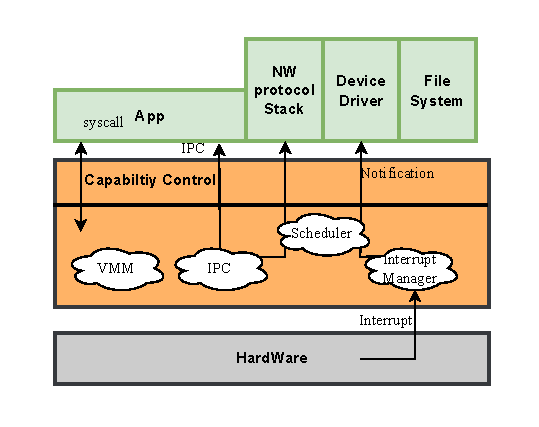
\includegraphics[width=0.75\textwidth]{figures/seL4_framwork.drawio.pdf}
  \caption{seL4的系统结构图}\label{fig:seL4_frramework}
\end{figure*}

\subsection{内核对象与Capability机制}
seL4采用基于内核对象的能力(Capability)安全模型构建其访问控制体系。在该模型中,所有系统资源(如内存区域、通信端点等)都被抽象为内核对象,由内核统一管理其状态和生命周期。如表\ref{tab:kernel_object}所示,这些内核对象构成了系统资源的软件抽象,形成了系统状态的核心组成部分。

\begin{table*}[htbp]
  \centering
  \begin{tabular*}{1.0\textwidth}{@{\extracolsep{\fill}}ll}
  \toprule
    内核对象			&作用	 \\
  \midrule
    线程控制块(TCB)			&内核调度的基本单位,保存了用户任务运行所需的上下文。 \\
    能力空间(CSpace)			&访问能力的集合,维护了各个内核对象的访问能力和对应权限。	 \\
    地址空间(VSpace) &地址空间,维护了一段虚拟地址和物理地址的映射关系。	 \\
    物理页框(Frame)  &对应一个物理页,维护了物理页号和访问权限.\\
    端点(Endpoint)	&同步IPC的桥梁,维护了一个消息收发的状态机。 \\
    通知对象(Notification) &通知机制的桥梁,维护了一个通知状态位。\\
    无类型对象(Untyped)&物理内存管理的承载者,通过系统调用转化为其他内核对象。 \\
  \bottomrule
  \end{tabular*}
  \caption{seL4中的主要内核对象} \label{tab:kernel_object}
\end{table*}

为确保系统安全性,seL4实现了严格的访问隔离机制。用户态程序不能直接访问内核对象,而必须通过能力句柄(Capability handler)间接操作。每个能力句柄实际上是一个经过验证的引用,内核在其对应的Capability数据结构中维护了目标内核对象的物理地址及精确的访问权限集。当用户态发起系统调用时,内核会通过能力查找机制定位对应的Capability,进行权限验证后才会执行相应操作。这种显式的授权机制确保了所有资源访问都必须经过严格的权限检查。

Capability机制支持两种基本的权限传播方式:转移(Transfer)和派生(Derivation)。转移操作实现了权限的完全移交,原持有者将失去对应资源的访问权;而派生操作则允许创建具有受限权限的新Capability,这些权限必须是原Capability权限的真子集。通过这种派生关系,系统内自然形成了一个层次化的能力树(Capability Tree)结构。值得注意的是,该模型提供了动态的权限回收机制——任何父节点都可以通过revoke操作递归地撤销其所有子节点的访问权限。这种精密的权限传播与回收机制,使得seL4能够构建可验证的、最小特权原则的系统安全架构。

\subsection{内存管理架构}

seL4采用了一种创新的分离式内存管理架构,这种设计在保证系统安全性的同时,实现了管理权限的合理分配。如图\ref{fig:seL4_mm}所示,该架构将内存管理明确划分为两个层次:物理内存完全交由用户态管理,而虚拟内存则由内核态统一维护。这种分离式设计体现了微内核架构的最小特权原则,既降低了内核的复杂度,又为用户态提供了灵活的内存管理能力。

\begin{figure*}[htbp]
  \centering
  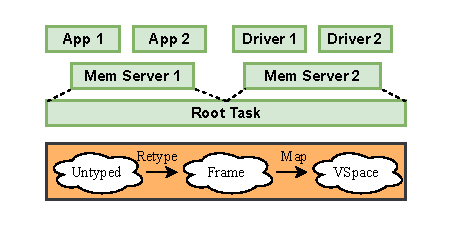
\includegraphics[width=0.75\textwidth]{figures/seL4_mm.drawio.pdf}
  \caption{seL4的内存管理}\label{fig:seL4_mm}
\end{figure*}

在物理内存管理方面,seL4引入了一种独特的Untyped对象机制。这些对象代表了系统初始化时可用的原始物理内存区域,具有以下重要特性:首先,它们在系统启动时由内核统一创建;其次,所有Untyped对象的能力都被集中授予Root Task用户进程;最后,用户态可以通过Retype系统调用对这些对象进行精细化操作。具体来说,Retype操作支持两种转换方式:一是将大块Untyped对象分割为更小的Untyped区域,二是将其转换为特定类型的内核对象(如Frame、CNodes等)。这种设计形成了一个完全由用户态主导的分布式递归内存管理体系,使得物理内存资源可以根据需要动态分配给不同的用户态组件。值得注意的是,这种机制不仅实现了物理内存的灵活管理,还通过能力系统确保了内存分配的安全性。

虚拟内存管理方面,seL4为每个进程维护一个VSpace内核对象,该对象作为地址空间的核心抽象,具有以下关键功能:它关联着进程的根页表结构,维护着完整的虚拟地址映射关系;它通过能力机制控制着地址空间的访问权限;它为内存隔离提供了硬件级的保护。用户态程序通过map/unmap系统调用可以动态调整Frame对象与虚拟地址的绑定关系,这些操作需要经过严格的能力检查。具体而言,map操作需要调用者同时拥有目标VSpace和Frame对象的能力,且映射范围必须在VSpace的有效区域内。这种设计既保证了内存访问的安全性,又为用户态提供了充分的灵活性。

这种分离式内存架构显著降低了内核的复杂度,将内存管理的策略性决策交由用户态实现,同时支持多种用户态内存管理策略的共存,不同的应用程序可以采用最适合自己的内存分配方案。这种架构设计不仅是内核最小化原则的体现,同时也是系统灵活性和可扩展性的重要支持。


\subsection{任务调度}
\label{sec:sel4_task}

seL4采用基于线程的轻量级任务调度模型,其设计体现了微内核架构的简约性和灵活性。在该模型中,线程作为最基本的执行单元和调度实体,包含了完整的执行上下文和独立的能力空间。值得注意的是,seL4对传统操作系统中的进程概念进行了弱化,通常情况下,我们将含有相同能力空间和地址空间的称为同一个进程,将进程抽象为资源分配的基本单位,因此在seL4中,进程只作为一个逻辑概念存在,内核的设计和实现只涉及到线程,这种设计选择使得内核实现更加精简,同时保持了足够的抽象能力来支持复杂的系统构建。

seL4的调度器实现采用了双层次的调度策略,将优先级调度与事件驱动的抢占调度有机结合。优先级调度基于经典的固定优先级算法,当出现以下两种情况时会触发调度决策:一是当前线程耗尽分配的时间片;二是线程因等待某些事件而主动阻塞。在调度时机到来时,内核会从就绪队列中选择优先级最高的线程进行上下文切换。另一方面,抢占调度机制主要应用于同步IPC场景,当线程间的通信操作导致更高优先级的线程变为可执行状态时,在不违反基本调度原则的前提下,内核会立即进行任务切换以保证系统的响应性。这种混合调度策略在保证系统确定性的同时,也优化了任务间的交互性能,具体的同步IPC流程描述参考\ref{sec:sel4_ipc}

\begin{figure*}[htbp]
  \centering
  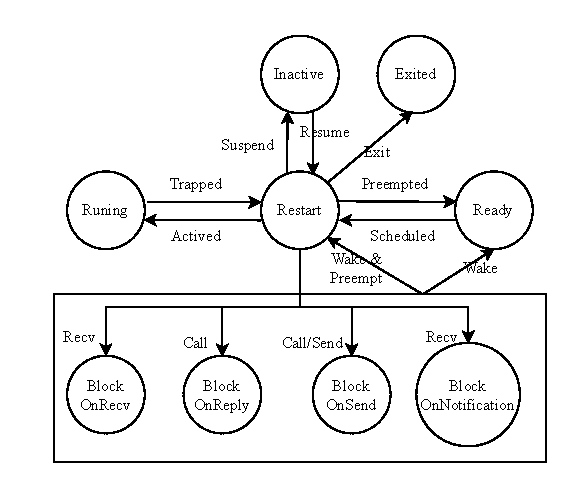
\includegraphics{figures/seL4_thread_state.drawio.pdf}
  \caption{seL4的线程状态转换}\label{fig:seL4_thread_state}
\end{figure*}

线程的状态转换图如\ref{fig:seL4_thread_state}所示,当线程陷入内核时,从Running切换为ReStart状态,即候选状态,当所有检查(如地址空间、优先级校验等)都通过了之后,从候选状态重新切换为Running状态并返回用户态,如果有更高优先级的线程存在,则会导致当前线程被抢占,转化为Ready状态,当检查出非法状态时,线程状态会被设置为Inactive,而在IPC通信过程中,可能会产生线程阻塞,此时根据不同的阻塞对象,线程状态会被设置为相应的阻塞状态。


为了满足实时系统的严格要求,seL4还提供了MCS(Mixed-Criticality Systems)扩展支持。该扩展通过三个关键机制来保证关键任务的实时性:首先,内核为关键任务预留专用的时间片资源;其次,系统支持运行时动态调整任务优先级;最后,MCS模式切换机制允许系统在不同关键性级别之间进行快速转换。

\subsection{同步IPC和通知机制}
\label{sec:sel4_ipc}
seL4微内核设计了一套完整的进程间通信(IPC)框架,该框架由同步IPC和异步通知机制共同构成,二者在语义和实现上存在显著差异。这种双模式设计使系统能够同时满足确定性通信和高效事件通知的需求。


同步IPC机制实现了严格的请求-响应语义,其核心特征在于通信双方的强同步性。如\ref{fig:seL4_ipc_state}所示,当客户端发起IPC调用时,系统会立即将调用线程阻塞,直至服务端完成请求处理并返回响应。这种同步性通过Endpoint内核对象实现,该对象维护着精确的状态机和阻塞队列。值得注意的是,同步IPC与任务调度器深度耦合,在通信过程中可能触发优先级驱动的任务切换。例如,当高优先级服务端线程被唤醒时,内核会立即执行上下文切换,这种设计保证了系统的时间确定性,使其特别适合需要严格时序保证的关键任务。

\begin{figure*}[htbp]
  \centering
  \includegraphics{figures/seL4_ipc_state.drawio.pdf}
  \caption{seL4的IPC相关内核对象状态转换}\label{fig:seL4_ipc_state}
\end{figure*}

相比之下,异步通知机制采用了完全不同的通信范式。该机制基于Notification内核对象实现,其最显著的特点是发送操作的异步性。通知发送方可以立即继续执行后续指令,而不需要等待接收方的响应。这种非阻塞特性显著提升了系统的并发处理能力,使其能够高效处理大量事件通知。然而,接收方仍然保持同步的接收模式,需要通过显式的系统调用获取通知内容。这种不对称设计在保证事件处理可靠性的同时,避免了纯异步模型可能带来的复杂性问题。

从实现层面看,两种机制的主要区别体现在三个方面:首先,同步IPC需要维护完整的调用上下文,而通知机制仅需管理信号位图;其次,同步IPC涉及双向数据传输,而通知主要是单向事件指示;最后,同步IPC会深度影响调度决策,而通知对系统调度的影响相对有限。


\subsection{中断管理与SMP支持}
seL4在中断管理与对称多处理机(SMP)支持方面也与主流内核有所区别,seL4为了保证内核行为的可预测性,在内核中屏蔽了所有外部中断,禁止内核中的中断抢占,这是由于seL4中的大部分内核任务都极其简短,因此停留在内核中(屏蔽中断)的时间非常少,不会过多地影响系统的实时性,而对于少量可能造成内核执行时间较长的系统调用,seL4在这些系统调用中插入了可抢占点,将内核的行为约束在可控范围内。

出于同样的目的,对于多CPU核心系统,seL4通过内核锁保证只有一个核心运行在内核态,避免了复杂的内核资源竞争,同时保证了内核行为的可预测性,大部分的系统调用都只会短暂停留在内核中,一般不会出现饥饿等待的情况,而对于少量可能造成内核执行时间较长的系统调用,seL4在流程中添加重启点,保存少量用于指示当前执行状态的信息,然后释放内核锁,等待下一次获取内核锁之后重启流程,以此避免饥饿等待的发生。

\subsection{本章小节}
本章系统地分析了seL4微内核的关键架构设计及其实现机制。作为第三代微内核的代表,seL4通过精心的架构设计在安全性、可靠性和性能之间取得了卓越的平衡。

在核心抽象层面,seL4采用了基于能力(Capability)的安全模型,所有系统资源都被封装为内核对象,并通过严格的能力机制进行访问控制。这种设计不仅实现了最小特权原则,还通过能力派生树(Capability Tree)支持灵活的权限管理。特别值得注意的是,能力机制与内核对象模型的紧密结合,构成了seL4安全架构的理论基础。

内存管理方面,seL4创新性地采用了物理内存与虚拟内存分离管理的架构。通过Untyped对象和Retype机制,系统实现了用户态主导的物理内存分配,而内核则专注于虚拟地址空间的维护。这种分离式设计既保证了内存访问的安全性,又为用户态提供了充分的灵活性,支持多种内存管理策略的并存实现。

任务调度模型体现了seL4对实时性的重视。系统将线程作为基本调度单元,弱化了传统进程概念,同时实现了优先级调度与事件驱动抢占调度的有机结合。MCS扩展进一步增强了系统的实时性保证,通过时间片预留和动态优先级调整等机制,满足了混合关键性系统的严格要求。

在进程间通信方面,seL4的双模式IPC框架展现了出色的设计平衡。同步IPC机制通过Endpoint对象实现严格的请求-响应语义,与任务调度深度集成;而异步通知机制则基于Notification对象,提供了高效的事件通知能力。这两种通信模式的协同工作,使系统能够同时满足确定性通信和高并发处理的需求。

尽管seL4微内核在设计上取得了显著成就,但其架构仍存在若干值得关注的技术局限性。首先,内核中同时维护同步IPC和异步通知两套通信机制,这一设计选择实质上违反了微内核架构的最小化原则。从实现复杂度来看,这两种机制需要分别维护Endpoint和Notification两类内核对象,以及各自对应的状态管理逻辑,导致内核代码量增加,更关键的是,这种双机制设计使得内核的验证复杂度呈指数级增长,造成形式化验证的工作量增加。其次,在性能开销方面,无论同步还是异步通信都需要陷入内核态进行处理,这种开销在频繁通信场景下会显著影响系统整体性能,特别是在云计算等对延迟敏感的应用中,可能造成较高的吞吐量下降。

